
%% bare_adv.tex
%% V1.4
%% 2012/12/27
%% by Michael Shell
%% See: 
%% http://www.michaelshell.org/
%% for current contact information.
%%
%% This is a skeleton file demonstrating the advanced use of IEEEtran.cls
%% (requires IEEEtran.cls version 1.8 or later) with an IEEE Computer
%% Society journal paper.
%%
%% Support sites:
%% http://www.michaelshell.org/tex/ieeetran/
%% http://www.ctan.org/tex-archive/macros/latex/contrib/IEEEtran/
%% and
%% http://www.ieee.org/

%%*************************************************************************
%% Legal Notice:
%% This code is offered as-is without any warranty either expressed or
%% implied; without even the implied warranty of MERCHANTABILITY or
%% FITNESS FOR A PARTICULAR PURPOSE! 
%% User assumes all risk.
%% In no event shall IEEE or any contributor to this code be liable for
%% any damages or losses, including, but not limited to, incidental,
%% consequential, or any other damages, resulting from the use or misuse
%% of any information contained here.
%%
%% All comments are the opinions of their respective authors and are not
%% necessarily endorsed by the IEEE.
%%
%% This work is distributed under the LaTeX Project Public License (LPPL)
%% ( http://www.latex-project.org/ ) version 1.3, and may be freely used,
%% distributed and modified. A copy of the LPPL, version 1.3, is included
%% in the base LaTeX documentation of all distributions of LaTeX released
%% 2003/12/01 or later.
%% Retain all contribution notices and credits.
%% ** Modified files should be clearly indicated as such, including  **
%% ** renaming them and changing author support contact information. **
%%
%% File list of work: IEEEtran.cls, IEEEtran_HOWTO.pdf, bare_adv.tex,
%%                    bare_conf.tex, bare_jrnl.tex, bare_jrnl_compsoc.tex,
%%                    bare_jrnl_transmag.tex
%%*************************************************************************

% *** Authors should verify (and, if needed, correct) their LaTeX system  ***
% *** with the testflow diagnostic prior to trusting their LaTeX platform ***
% *** with production work. IEEE's font choices can trigger bugs that do  ***
% *** not appear when using other class files.                            ***
% The testflow support page is at:
% http://www.michaelshell.org/tex/testflow/



% IEEEtran V1.7 and later provides for these CLASSINPUT macros to allow the
% user to reprogram some IEEEtran.cls defaults if needed. These settings
% override the internal defaults of IEEEtran.cls regardless of which class
% options are used. Do not use these unless you have good reason to do so as
% they can result in nonIEEE compliant documents. User beware. ;)
%
%\newcommand{\CLASSINPUTbaselinestretch}{1.0} % baselinestretch
%\newcommand{\CLASSINPUTinnersidemargin}{1in} % inner side margin
%\newcommand{\CLASSINPUToutersidemargin}{1in} % outer side margin
%\newcommand{\CLASSINPUTtoptextmargin}{1in}   % top text margin
%\newcommand{\CLASSINPUTbottomtextmargin}{1in}% bottom text margin



% Note that the a4paper option is mainly intended so that authors in
% countries using A4 can easily print to A4 and see how their papers will
% look in print - the typesetting of the document will not typically be
% affected with changes in paper size (but the bottom and side margins will).
% Use the testflow package mentioned above to verify correct handling of
% both paper sizes by the user's LaTeX system.
%
% Also note that the "draftcls" or "draftclsnofoot", not "draft", option
% should be used if it is desired that the figures are to be displayed in
% draft mode.
%
\documentclass[12pt,journal,compsoc]{IEEEtran}
% The Computer Society requires 12pt.
% If IEEEtran.cls has not been installed into the LaTeX system files,
% manually specify the path to it like:
% \documentclass[10pt,journal,compsoc]{../sty/IEEEtran}


% For Computer Society journals, IEEEtran defaults to the use of 
% Palatino/Palladio as is done in IEEE Computer Society journals.
% To go back to Times Roman, you can use this code:
%\renewcommand{\rmdefault}{ptm}\selectfont





% Some very useful LaTeX packages include:
% (uncomment the ones you want to load)



% *** MISC UTILITY PACKAGES ***
%
%\usepackage{ifpdf}
% Heiko Oberdiek's ifpdf.sty is very useful if you need conditional
% compilation based on whether the output is pdf or dvi.
% usage:
% \ifpdf
%   % pdf code
% \else
%   % dvi code
% \fi
% The latest version of ifpdf.sty can be obtained from:
% http://www.ctan.org/tex-archive/macros/latex/contrib/oberdiek/
% Also, note that IEEEtran.cls V1.7 and later provides a builtin
% \ifCLASSINFOpdf conditional that works the same way.
% When switching from latex to pdflatex and vice-versa, the compiler may
% have to be run twice to clear warning/error messages.






% *** CITATION PACKAGES ***
%
\ifCLASSOPTIONcompsoc
  % IEEE Computer Society needs nocompress option
  % requires cite.sty v4.0 or later (November 2003)
  % \usepackage[nocompress]{cite}
\else
  % normal IEEE
  % \usepackage{cite}
\fi
% cite.sty was written by Donald Arseneau
% V1.6 and later of IEEEtran pre-defines the format of the cite.sty package
% \cite{} output to follow that of IEEE. Loading the cite package will
% result in citation numbers being automatically sorted and properly
% "compressed/ranged". e.g., [1], [9], [2], [7], [5], [6] without using
% cite.sty will become [1], [2], [5]--[7], [9] using cite.sty. cite.sty's
% \cite will automatically add leading space, if needed. Use cite.sty's
% noadjust option (cite.sty V3.8 and later) if you want to turn this off
% such as if a citation ever needs to be enclosed in parenthesis.
% cite.sty is already installed on most LaTeX systems. Be sure and use
% version 4.0 (2003-05-27) and later if using hyperref.sty. cite.sty does
% not currently provide for hyperlinked citations.
% The latest version can be obtained at:
% http://www.ctan.org/tex-archive/macros/latex/contrib/cite/
% The documentation is contained in the cite.sty file itself.
%
% Note that some packages require special options to format as the Computer
% Society requires. In particular, Computer Society  papers do not use
% compressed citation ranges as is done in typical IEEE papers
% (e.g., [1]-[4]). Instead, they list every citation separately in order
% (e.g., [1], [2], [3], [4]). To get the latter we need to load the cite
% package with the nocompress option which is supported by cite.sty v4.0
% and later.
%
% Note also the use of a CLASSOPTION conditional provided by 
% IEEEtran.cls V1.7 and later.





% *** GRAPHICS RELATED PACKAGES ***
%
\ifCLASSINFOpdf
  \usepackage[pdftex]{graphicx}
  % declare the path(s) where your graphic files are
  % \graphicspath{{../pdf/}{../jpeg/}}
  % and their extensions so you won't have to specify these with
  % every instance of \includegraphics
  % \DeclareGraphicsExtensions{.pdf,.jpeg,.png}
\else
  % or other class option (dvipsone, dvipdf, if not using dvips). graphicx
  % will default to the driver specified in the system graphics.cfg if no
  % driver is specified.
  % \usepackage[dvips]{graphicx}
  % declare the path(s) where your graphic files are
  % \graphicspath{{../eps/}}
  % and their extensions so you won't have to specify these with
  % every instance of \includegraphics
  % \DeclareGraphicsExtensions{.eps}
\fi
% graphicx was written by David Carlisle and Sebastian Rahtz. It is
% required if you want graphics, photos, etc. graphicx.sty is already
% installed on most LaTeX systems. The latest version and documentation
% can be obtained at: 
% http://www.ctan.org/tex-archive/macros/latex/required/graphics/
% Another good source of documentation is "Using Imported Graphics in
% LaTeX2e" by Keith Reckdahl which can be found at:
% http://www.ctan.org/tex-archive/info/epslatex/
%
% latex, and pdflatex in dvi mode, support graphics in encapsulated
% postscript (.eps) format. pdflatex in pdf mode supports graphics
% in .pdf, .jpeg, .png and .mps (metapost) formats. Users should ensure
% that all non-photo figures use a vector format (.eps, .pdf, .mps) and
% not a bitmapped formats (.jpeg, .png). IEEE frowns on bitmapped formats
% which can result in "jaggedy"/blurry rendering of lines and letters as
% well as large increases in file sizes.
%
% You can find documentation about the pdfTeX application at:
% http://www.tug.org/applications/pdftex





% *** MATH PACKAGES ***
%
\usepackage[cmex10]{amsmath}
% A popular package from the American Mathematical Society that provides
% many useful and powerful commands for dealing with mathematics. If using
% it, be sure to load this package with the cmex10 option to ensure that
% only type 1 fonts will utilized at all point sizes. Without this option,
% it is possible that some math symbols, particularly those within
% footnotes, will be rendered in bitmap form which will result in a
% document that can not be IEEE Xplore compliant!
%
% Also, note that the amsmath package sets \interdisplaylinepenalty to 10000
% thus preventing page breaks from occurring within multiline equations. Use:
%\interdisplaylinepenalty=2500
% after loading amsmath to restore such page breaks as IEEEtran.cls normally
% does. amsmath.sty is already installed on most LaTeX systems. The latest
% version and documentation can be obtained at:
% http://www.ctan.org/tex-archive/macros/latex/required/amslatex/math/





% *** SPECIALIZED LIST PACKAGES ***
%\usepackage{acronym}
% acronym.sty was written by Tobias Oetiker. This package provides tools for
% managing documents with large numbers of acronyms. (You don't *have* to
% use this package - unless you have a lot of acronyms, you may feel that
% such package management of them is bit of an overkill.)
% Do note that the acronym environment (which lists acronyms) will have a
% problem when used under IEEEtran.cls because acronym.sty relies on the
% description list environment - which IEEEtran.cls has customized for
% producing IEEE style lists. A workaround is to declared the longest
% label width via the IEEEtran.cls \IEEEiedlistdecl global control:
%
% \renewcommand{\IEEEiedlistdecl}{\IEEEsetlabelwidth{SONET}}
% \begin{acronym}
%
% \end{acronym}
% \renewcommand{\IEEEiedlistdecl}{\relax}% remember to reset \IEEEiedlistdecl
%
% instead of using the acronym environment's optional argument.
% The latest version and documentation can be obtained at:
% http://www.ctan.org/tex-archive/macros/latex/contrib/acronym/


%\usepackage{algorithmic}
% algorithmic.sty was written by Peter Williams and Rogerio Brito.
% This package provides an algorithmic environment fo describing algorithms.
% You can use the algorithmic environment in-text or within a figure
% environment to provide for a floating algorithm. Do NOT use the algorithm
% floating environment provided by algorithm.sty (by the same authors) or
% algorithm2e.sty (by Christophe Fiorio) as IEEE does not use dedicated
% algorithm float types and packages that provide these will not provide
% correct IEEE style captions. The latest version and documentation of
% algorithmic.sty can be obtained at:
% http://www.ctan.org/tex-archive/macros/latex/contrib/algorithms/
% There is also a support site at:
% http://algorithms.berlios.de/index.html
% Also of interest may be the (relatively newer and more customizable)
% algorithmicx.sty package by Szasz Janos:
% http://www.ctan.org/tex-archive/macros/latex/contrib/algorithmicx/




% *** ALIGNMENT PACKAGES ***
%
%\usepackage{array}
% Frank Mittelbach's and David Carlisle's array.sty patches and improves
% the standard LaTeX2e array and tabular environments to provide better
% appearance and additional user controls. As the default LaTeX2e table
% generation code is lacking to the point of almost being broken with
% respect to the quality of the end results, all users are strongly
% advised to use an enhanced (at the very least that provided by array.sty)
% set of table tools. array.sty is already installed on most systems. The
% latest version and documentation can be obtained at:
% http://www.ctan.org/tex-archive/macros/latex/required/tools/


%\usepackage{mdwmath}
%\usepackage{mdwtab}
% Also highly recommended is Mark Wooding's extremely powerful MDW tools,
% especially mdwmath.sty and mdwtab.sty which are used to format equations
% and tables, respectively. The MDWtools set is already installed on most
% LaTeX systems. The lastest version and documentation is available at:
% http://www.ctan.org/tex-archive/macros/latex/contrib/mdwtools/


% IEEEtran contains the IEEEeqnarray family of commands that can be used to
% generate multiline equations as well as matrices, tables, etc., of high
% quality.


%\usepackage{eqparbox}
% Also of notable interest is Scott Pakin's eqparbox package for creating
% (automatically sized) equal width boxes - aka "natural width parboxes".
% Available at:
% http://www.ctan.org/tex-archive/macros/latex/contrib/eqparbox/




% *** SUBFIGURE PACKAGES ***
%\ifCLASSOPTIONcompsoc
%  \usepackage[caption=false,font=normalsize,labelfont=sf,textfont=sf]{subfig}
%\else
%  \usepackage[caption=false,font=footnotesize]{subfig}
%\fi
% subfig.sty, written by Steven Douglas Cochran, is the modern replacement
% for subfigure.sty, the latter of which is no longer maintained and is
% incompatible with some LaTeX packages including fixltx2e. However,
% subfig.sty requires and automatically loads Axel Sommerfeldt's caption.sty
% which will override IEEEtran.cls' handling of captions and this will result
% in non-IEEE style figure/table captions. To prevent this problem, be sure
% and invoke subfig.sty's "caption=false" package option (available since
% subfig.sty version 1.3, 2005/06/28) as this is will preserve IEEEtran.cls
% handling of captions.
% Note that the Computer Society format requires a larger sans serif font
% than the serif footnote size font used in traditional IEEE formatting
% and thus the need to invoke different subfig.sty package options depending
% on whether compsoc mode has been enabled.
%
% The latest version and documentation of subfig.sty can be obtained at:
% http://www.ctan.org/tex-archive/macros/latex/contrib/subfig/




% *** FLOAT PACKAGES ***
%
%\usepackage{fixltx2e}
% fixltx2e, the successor to the earlier fix2col.sty, was written by
% Frank Mittelbach and David Carlisle. This package corrects a few problems
% in the LaTeX2e kernel, the most notable of which is that in current
% LaTeX2e releases, the ordering of single and double column floats is not
% guaranteed to be preserved. Thus, an unpatched LaTeX2e can allow a
% single column figure to be placed prior to an earlier double column
% figure. The latest version and documentation can be found at:
% http://www.ctan.org/tex-archive/macros/latex/base/


%\usepackage{stfloats}
% stfloats.sty was written by Sigitas Tolusis. This package gives LaTeX2e
% the ability to do double column floats at the bottom of the page as well
% as the top. (e.g., "\begin{figure*}[!b]" is not normally possible in
% LaTeX2e). It also provides a command:
%\fnbelowfloat
% to enable the placement of footnotes below bottom floats (the standard
% LaTeX2e kernel puts them above bottom floats). This is an invasive package
% which rewrites many portions of the LaTeX2e float routines. It may not work
% with other packages that modify the LaTeX2e float routines. The latest
% version and documentation can be obtained at:
% http://www.ctan.org/tex-archive/macros/latex/contrib/sttools/
% Do not use the stfloats baselinefloat ability as IEEE does not allow
% \baselineskip to stretch. Authors submitting work to the IEEE should note
% that IEEE rarely uses double column equations and that authors should try
% to avoid such use. Do not be tempted to use the cuted.sty or midfloat.sty
% packages (also by Sigitas Tolusis) as IEEE does not format its papers in
% such ways.
% Do not attempt to use stfloats with fixltx2e as they are incompatible.
% Instead, use Morten Hogholm'a dblfloatfix which combines the features
% of both fixltx2e and stfloats:
%
% \usepackage{dblfloatfix}
% The latest version can be found at:
% http://www.ctan.org/tex-archive/macros/latex/contrib/dblfloatfix/


%\ifCLASSOPTIONcaptionsoff
%  \usepackage[nomarkers]{endfloat}
% \let\MYoriglatexcaption\caption
% \renewcommand{\caption}[2][\relax]{\MYoriglatexcaption[#2]{#2}}
%\fi
% endfloat.sty was written by James Darrell McCauley, Jeff Goldberg and 
% Axel Sommerfeldt. This package may be useful when used in conjunction with 
% IEEEtran.cls'  captionsoff option. Some IEEE journals/societies require that
% submissions have lists of figures/tables at the end of the paper and that
% figures/tables without any captions are placed on a page by themselves at
% the end of the document. If needed, the draftcls IEEEtran class option or
% \CLASSINPUTbaselinestretch interface can be used to increase the line
% spacing as well. Be sure and use the nomarkers option of endfloat to
% prevent endfloat from "marking" where the figures would have been placed
% in the text. The two hack lines of code above are a slight modification of
% that suggested by in the endfloat docs (section 8.4.1) to ensure that
% the full captions always appear in the list of figures/tables - even if
% the user used the short optional argument of \caption[]{}.
% IEEE papers do not typically make use of \caption[]'s optional argument,
% so this should not be an issue. A similar trick can be used to disable
% captions of packages such as subfig.sty that lack options to turn off
% the subcaptions:
% For subfig.sty:
% \let\MYorigsubfloat\subfloat
% \renewcommand{\subfloat}[2][\relax]{\MYorigsubfloat[]{#2}}
% However, the above trick will not work if both optional arguments of
% the \subfloat command are used. Furthermore, there needs to be a
% description of each subfigure *somewhere* and endfloat does not add
% subfigure captions to its list of figures. Thus, the best approach is to
% avoid the use of subfigure captions (many IEEE journals avoid them anyway)
% and instead reference/explain all the subfigures within the main caption.
% The latest version of endfloat.sty and its documentation can obtained at:
% http://www.ctan.org/tex-archive/macros/latex/contrib/endfloat/
%
% The IEEEtran \ifCLASSOPTIONcaptionsoff conditional can also be used
% later in the document, say, to conditionally put the References on a 
% page by themselves.





% *** PDF, URL AND HYPERLINK PACKAGES ***
%
%\usepackage{url}
% url.sty was written by Donald Arseneau. It provides better support for
% handling and breaking URLs. url.sty is already installed on most LaTeX
% systems. The latest version and documentation can be obtained at:
% http://www.ctan.org/tex-archive/macros/latex/contrib/url/
% Basically, \url{my_url_here}.


% NOTE: PDF thumbnail features are not required in IEEE papers
%       and their use requires extra complexity and work.
%\ifCLASSINFOpdf
%  \usepackage[pdftex]{thumbpdf}
%\else
%  \usepackage[dvips]{thumbpdf}
%\fi
% thumbpdf.sty and its companion Perl utility were written by Heiko Oberdiek.
% It allows the user a way to produce PDF documents that contain fancy
% thumbnail images of each of the pages (which tools like acrobat reader can
% utilize). This is possible even when using dvi->ps->pdf workflow if the
% correct thumbpdf driver options are used. thumbpdf.sty incorporates the
% file containing the PDF thumbnail information (filename.tpm is used with
% dvips, filename.tpt is used with pdftex, where filename is the base name of
% your tex document) into the final ps or pdf output document. An external
% utility, the thumbpdf *Perl script* is needed to make these .tpm or .tpt
% thumbnail files from a .ps or .pdf version of the document (which obviously
% does not yet contain pdf thumbnails). Thus, one does a:
% 
% thumbpdf filename.pdf 
%
% to make a filename.tpt, and:
%
% thumbpdf --mode dvips filename.ps
%
% to make a filename.tpm which will then be loaded into the document by
% thumbpdf.sty the NEXT time the document is compiled (by pdflatex or
% latex->dvips->ps2pdf). Users must be careful to regenerate the .tpt and/or
% .tpm files if the main document changes and then to recompile the
% document to incorporate the revised thumbnails to ensure that thumbnails
% match the actual pages. It is easy to forget to do this!
% 
% Unix systems come with a Perl interpreter. However, MS Windows users
% will usually have to install a Perl interpreter so that the thumbpdf
% script can be run. The Ghostscript PS/PDF interpreter is also required.
% See the thumbpdf docs for details. The latest version and documentation
% can be obtained at.
% http://www.ctan.org/tex-archive/support/thumbpdf/


% NOTE: PDF hyperlink and bookmark features are not required in IEEE
%       papers and their use requires extra complexity and work.
% *** IF USING HYPERREF BE SURE AND CHANGE THE EXAMPLE PDF ***
% *** TITLE/SUBJECT/AUTHOR/KEYWORDS INFO BELOW!!           ***
\newcommand\MYhyperrefoptions{bookmarks=true,bookmarksnumbered=true,
pdfpagemode={UseOutlines},plainpages=false,pdfpagelabels=true,
colorlinks=true,linkcolor={black},citecolor={black},urlcolor={black},
pdftitle={Bare Demo of IEEEtran.cls for Computer Society Journals},%<!CHANGE!
pdfsubject={Typesetting},%<!CHANGE!
pdfauthor={David Ocepek},%<!CHANGE!
pdfkeywords={Computer Society, IEEEtran, journal, LaTeX, paper,
             template}}%<^!CHANGE!
%\ifCLASSINFOpdf
%\usepackage[\MYhyperrefoptions,pdftex]{hyperref}
%\else
%\usepackage[\MYhyperrefoptions,breaklinks=true,dvips]{hyperref}
%\usepackage{breakurl}
%\fi
% One significant drawback of using hyperref under DVI output is that the
% LaTeX compiler cannot break URLs across lines or pages as can be done
% under pdfLaTeX's PDF output via the hyperref pdftex driver. This is
% probably the single most important capability distinction between the
% DVI and PDF output. Perhaps surprisingly, all the other PDF features
% (PDF bookmarks, thumbnails, etc.) can be preserved in
% .tex->.dvi->.ps->.pdf workflow if the respective packages/scripts are
% loaded/invoked with the correct driver options (dvips, etc.). 
% As most IEEE papers use URLs sparingly (mainly in the references), this
% may not be as big an issue as with other publications.
%
% That said, Vilar Camara Neto created his breakurl.sty package which
% permits hyperref to easily break URLs even in dvi mode.
% Note that breakurl, unlike most other packages, must be loaded
% AFTER hyperref. The latest version of breakurl and its documentation can
% be obtained at:
% http://www.ctan.org/tex-archive/macros/latex/contrib/breakurl/
% breakurl.sty is not for use under pdflatex pdf mode.
%
% The advanced features offer by hyperref.sty are not required for IEEE
% submission, so users should weigh these features against the added
% complexity of use.
% The package options above demonstrate how to enable PDF bookmarks
% (a type of table of contents viewable in Acrobat Reader) as well as
% PDF document information (title, subject, author and keywords) that is
% viewable in Acrobat reader's Document_Properties menu. PDF document
% information is also used extensively to automate the cataloging of PDF
% documents. The above set of options ensures that hyperlinks will not be
% colored in the text and thus will not be visible in the printed page,
% but will be active on "mouse over". USING COLORS OR OTHER HIGHLIGHTING
% OF HYPERLINKS CAN RESULT IN DOCUMENT REJECTION BY THE IEEE, especially if
% these appear on the "printed" page. IF IN DOUBT, ASK THE RELEVANT
% SUBMISSION EDITOR. You may need to add the option hypertexnames=false if
% you used duplicate equation numbers, etc., but this should not be needed
% in normal IEEE work.
% The latest version of hyperref and its documentation can be obtained at:
% http://www.ctan.org/tex-archive/macros/latex/contrib/hyperref/





% *** Do not adjust lengths that control margins, column widths, etc. ***
% *** Do not use packages that alter fonts (such as pslatex).         ***
% There should be no need to do such things with IEEEtran.cls V1.6 and later.
% (Unless specifically asked to do so by the journal or conference you plan
% to submit to, of course. )
\usepackage{float}

% correct bad hyphenation here
\hyphenation{op-tical net-works semi-conduc-tor}

\DeclareMathOperator*{\argmax}{arg\,max}
\DeclareMathOperator*{\argmin}{arg\,min}
\newcommand{\Lagr}{\mathcal{L}}

\begin{document}
%
% paper title
% can use linebreaks \\ within to get better formatting as desired
% Do not put math or special symbols in the title.
\title{Stock Price Prediction using LSTM, CNN, CNN-LSTM and ARIMA}
%
%
% author names and IEEE memberships
% note positions of commas and nonbreaking spaces ( ~ ) LaTeX will not break
% a structure at a ~ so this keeps an author's name from being broken across
% two lines.
% use \thanks{} to gain access to the first footnote area
% a separate \thanks must be used for each paragraph as LaTeX2e's \thanks
% was not built to handle multiple paragraphs
%
%
%\IEEEcompsocitemizethanks is a special \thanks that produces the bulleted
% lists the Computer Society journals use for "first footnote" author
% affiliations. Use \IEEEcompsocthanksitem which works much like \item
% for each affiliation group. When not in compsoc mode,
% \IEEEcompsocitemizethanks becomes like \thanks and
% \IEEEcompsocthanksitem becomes a line break with idention. This
% facilitates dual compilation, although admittedly the differences in the
% desired content of \author between the different types of papers makes a
% one-size-fits-all approach a daunting prospect. For instance, compsoc 
% journal papers have the author affiliations above the "Manuscript
% received ..."  text while in non-compsoc journals this is reversed. Sigh.

%\author{David~Ocepek% <-this % stops a space
%\IEEEcompsocitemizethanks{\IEEEcompsocthanksitem M. Shell is with the Department
%of Electrical and Computer Engineering, Georgia Institute of Technology, Atlanta,
%GA, 30332.\protect\\
% note need leading \protect in front of \\ to get a newline within \thanks as
% \\ is fragile and will error, could use \hfil\break instead.
% E-mail: see http://www.michaelshell.org/contact.html
%\IEEEcompsocthanksitem J. Doe and J. Doe are with Anonymous University.}% <-this % stops a space
%\thanks{Manuscript received April 19, 2005; revised December 27, 2012.}}

% note the % following the last \IEEEmembership and also \thanks - 
% these prevent an unwanted space from occurring between the last author name
% and the end of the author line. i.e., if you had this:
% 
% \author{....lastname \thanks{...} \thanks{...} }
%                     ^------------^------------^----Do not want these spaces!
%
% a space would be appended to the last name and could cause every name on that
% line to be shifted left slightly. This is one of those "LaTeX things". For
% instance, "\textbf{A} \textbf{B}" will typeset as "A B" not "AB". To get
% "AB" then you have to do: "\textbf{A}\textbf{B}"
% \thanks is no different in this regard, so shield the last } of each \thanks
% that ends a line with a % and do not let a space in before the next \thanks.
% Spaces after \IEEEmembership other than the last one are OK (and needed) as
% you are supposed to have spaces between the names. For what it is worth,
% this is a minor point as most people would not even notice if the said evil
% space somehow managed to creep in.


\author{David~Ocepek}% <-this % stops a space

% The paper headers
\markboth{Machine Learning Course Seminar project, December~2021}%
{Shell \MakeLowercase{\textit{et al.}}: Bare Advanced Demo of IEEEtran.cls for Journals}
% The only time the second header will appear is for the odd numbered pages
% after the title page when using the twoside option.
% 
% *** Note that you probably will NOT want to include the author's ***
% *** name in the headers of peer review papers.                   ***
% You can use \ifCLASSOPTIONpeerreview for conditional compilation here if
% you desire.



% The publisher's ID mark at the bottom of the page is less important with
% Computer Society journal papers as those publications place the marks
% outside of the main text columns and, therefore, unlike regular IEEE
% journals, the available text space is not reduced by their presence.
% If you want to put a publisher's ID mark on the page you can do it like
% this:
%\IEEEpubid{0000--0000/00\$00.00~\copyright~2012 IEEE}
% or like this to get the Computer Society new two part style.
%\IEEEpubid{\makebox[\columnwidth]{\hfill 0000--0000/00/\$00.00~\copyright~2012 IEEE}%
%\hspace{\columnsep}\makebox[\columnwidth]{Published by the IEEE Computer Society\hfill}}
% Remember, if you use this you must call \IEEEpubidadjcol in the second
% column for its text to clear the IEEEpubid mark (Computer Society journal
% papers don't need this extra clearance.)



% use for special paper notices
%\IEEEspecialpapernotice{(Invited Paper)}



% for Computer Society papers, we must declare the abstract and index terms
% PRIOR to the title within the \IEEEtitleabstractindextext IEEEtran
% command as these need to go into the title area created by \maketitle.
% As a general rule, do not put math, special symbols or citations
% in the abstract or keywords.
\IEEEtitleabstractindextext{%
\begin{abstract}
Stock price forecasting is a long-term area of interest for the financial world with many new models being proposed on a monthly basis.
In this paper we conducted a comparative analysis of LSTM, CNN, CNN-LSTM and ARIMA on five tech stock data sets obtained from YAHOO! Finance.
We built upon our analysis by using ARIMA to remove seasonality and trend from our time series and analyzed the room for improvement that hybrid models, such as ARIMA-CNN can offer.
We used our models to predict the next day opening price of each stock and quantified the stability of our results using cross-validation on a rolling basis. 
Our results show that ARIMA is overall the best model for short-term time series forecasting compared to non-hybrid models, furthermore it
appears that we can improve ARIMA models by using CNNs or CNN-LSTMs to reduce residual errors of the ARIMA model.

\end{abstract}

% Note that keywords are not normally used for peerreview papers.
\begin{IEEEkeywords}
Stock price forecasting, ARIMA model, convolutional neural networks(CNN), Long Short-term memory networks(LSTM),
convolutional long short-term memory(CNN-LSTM), hybrid models 
\end{IEEEkeywords}}


% make the title area
\maketitle


% To allow for easy dual compilation without having to reenter the
% abstract/keywords data, the \IEEEtitleabstractindextext text will
% not be used in maketitle, but will appear (i.e., to be "transported")
% here as \IEEEdisplaynontitleabstractindextext when compsoc mode
% is not selected <OR> if conference mode is selected - because compsoc
% conference papers position the abstract like regular (non-compsoc)
% papers do!
\IEEEdisplaynontitleabstractindextext
% \IEEEdisplaynontitleabstractindextext has no effect when using
% compsoc under a non-conference mode.


% For peer review papers, you can put extra information on the cover
% page as needed:
% \ifCLASSOPTIONpeerreview
% \begin{center} \bfseries EDICS Category: 3-BBND \end{center}
% \fi
%
% For peerreview papers, this IEEEtran command inserts a page break and
% creates the second title. It will be ignored for other modes.
\IEEEpeerreviewmaketitle



\section{Introduction}
% Computer Society journal papers do something a tad strange with the very
% first section heading (almost always called "Introduction"). They place it
% ABOVE the main text! IEEEtran.cls currently does not do this for you.
% However, You can achieve this effect by making LaTeX jump through some
% hoops via something like:
%
%\ifCLASSOPTIONcompsoc
%  \noindent\raisebox{2\baselineskip}[0pt][0pt]%
%  {\parbox{\columnwidth}{\section{Introduction}\label{sec:introduction}%
%  \global\everypar=\everypar}}%
%  \vspace{-1\baselineskip}\vspace{-\parskip}\par
%\else
%  \section{Introduction}\label{sec:introduction}\par
%\fi
%
% Admittedly, this is a hack and may well be fragile, but seems to do the
% trick for me. Note the need to keep any \label that may be used right
% after \section in the above as the hack puts \section within a raised box.



% The very first letter is a 2 line initial drop letter followed
% by the rest of the first word in caps (small caps for compsoc).
% 
% form to use if the first word consists of a single letter:
% \IEEEPARstart{A}{demo} file is ....
% 
% form to use if you need the single drop letter followed by
% normal text (unknown if ever used by IEEE):
% \IEEEPARstart{A}{}demo file is ....
% 
% Some journals put the first two words in caps:
% \IEEEPARstart{T}{his demo} file is ....
% 
% Here we have the typical use of a "T" for an initial drop letter
% and "HIS" in caps to complete the first word.
\IEEEPARstart{A}{utomated} stock trading systems are commonly used in the financial sector to maximize profits by optimizing stock prediction models.
For example, in 2016 more than 80\% of transactions in the Forex market were directed by robots~\cite{intro-forex}.
Because of widespread automatization even small improvements in model prediction accuracy would yield large profits for financial institutions.
This poses an interesting problem for data scientists because stock price forecasting is notoriously difficult due high levels of noise present in financial time series, a side-effect of market efficiency.
\par In our paper we focused on next-day opening price prediction using multiple neural network models.
As the baseline we used the statistical ARIMA model.
In addition, we conducted a comparative analysis of ARIMA-neural network hybrid models.
We explained and verified our results using the LIME algorithm.
\par Our contributions are minor and mainly in the domain of result reproducibility and improvement of hybrid model understanding by performing additional analysis in some less-analyzed areas such as quantification of model uncertainty with cross-validation on a rolling basis and cross-model comparison with LIME.

\subsection{Related Work}
\par Stock price forecasting is an actively researched field and a lot of work has been done in recent years to optimize stock price prediction.
Simpler models like ARIMA have lately been used to detrend and deseasonalize financial time series.
\par In 2017, Selvin et al.~\cite{selvin2017stock} used AR,ARMA and ARIMA to improve RNN, LSTM and CNN model predictions of closing prices of multiple NSE listed companies.
In 2019 Lei Ji et al.~\cite{carbon} used the ARIMA model to improve and analize carbon forecasting of CNN-LSTM.
In 2019 Hoseinzade et al.~\cite{HOSEINZADE2019273} used 3D CNNs to combine features from multiple markets to improve next-day direction of movement prediction of the S\&P 500, NASDAQ, DJI, NYSE and RUSSELL indices.
In 2020 Yan Wang et al.~\cite{wang2020forecasting} used an ARIMA XGBoost model to predict the opening price of 10 chinese stocks.
In 2021 Qi Tang et al.~\cite{ssa_transform} used Wavelet Transform (WT) and Singular Spectrum Analysis (SSA) to denoise the Dow Jones Industrial Average Index. This resulted in improved neural network prediction models.
In 2021 Xuan Ji et al.~\cite{word2vec} proposed using word2vec to build text feature vectors from social media and combining extracted features with stock market features as inputs to SSA smoothed LSTMs.

% needed in second column of first page if using \IEEEpubid
%\IEEEpubidadjcol

% An example of a floating figure using the graphicx package.
% Note that \label must occur AFTER (or within) \caption.
% For figures, \caption should occur after the \includegraphics.
% Note that IEEEtran v1.7 and later has special internal code that
% is designed to preserve the operation of \label within \caption
% even when the captionsoff option is in effect. However, because
% of issues like this, it may be the safest practice to put all your
% \label just after \caption rather than within \caption{}.
%
% Reminder: the "draftcls" or "draftclsnofoot", not "draft", class
% option should be used if it is desired that the figures are to be
% displayed while in draft mode.
%
%\begin{figure}[!t]
%\centering
%\includegraphics[width=2.5in]{myfigure}
% where an .eps filename suffix will be assumed under latex, 
% and a .pdf suffix will be assumed for pdflatex; or what has been declared
% via \DeclareGraphicsExtensions.
%\caption{Simulation Results.}
%\label{fig_sim}
%\end{figure}

% Note that IEEE typically puts floats only at the top, even when this
% results in a large percentage of a column being occupied by floats.
% However, the Computer Society has been known to put floats at the bottom.


% An example of a double column floating figure using two subfigures.
% (The subfig.sty package must be loaded for this to work.)
% The subfigure \label commands are set within each subfloat command,
% and the \label for the overall figure must come after \caption.
% \hfil is used as a separator to get equal spacing.
% Watch out that the combined width of all the subfigures on a 
% line do not exceed the text width or a line break will occur.
%
%\begin{figure*}[!t]
%\centering
%\subfloat[Case I]{\includegraphics[width=2.5in]{box}%
%\label{fig_first_case}}
%\hfil
%\subfloat[Case II]{\includegraphics[width=2.5in]{box}%
%\label{fig_second_case}}
%\caption{Simulation results.}
%\label{fig_sim}
%\end{figure*}
%
% Note that often IEEE papers with subfigures do not employ subfigure
% captions (using the optional argument to \subfloat[]), but instead will
% reference/describe all of them (a), (b), etc., within the main caption.


% An example of a floating table. Note that, for IEEE style tables, the 
% \caption command should come BEFORE the table. Table text will default to
% \footnotesize as IEEE normally uses this smaller font for tables.
% The \label must come after \caption as always.
%
%\begin{table}[!t]
%% increase table row spacing, adjust to taste
%\renewcommand{\arraystretch}{1.3}
% if using array.sty, it might be a good idea to tweak the value of
% \extrarowheight as needed to properly center the text within the cells
%\caption{An Example of a Table}
%\label{table_example}
%\centering
%% Some packages, such as MDW tools, offer better commands for making tables
%% than the plain LaTeX2e tabular which is used here.
%\begin{tabular}{|c||c|}
%\hline
%One & Two\\
%\hline
%Three & Four\\
%\hline
%\end{tabular}
%\end{table}


% Note that IEEE does not put floats in the very first column - or typically
% anywhere on the first page for that matter. Also, in-text middle ("here")
% positioning is not used. Most IEEE journals use top floats exclusively.
% However, Computer Society journals sometimes do use bottom floats - bear
% this in mind when choosing appropriate optional arguments for the
% figure/table environments.
% Note that, LaTeX2e, unlike IEEE journals, places footnotes above bottom
% floats. This can be corrected via the \fnbelowfloat command of the
% stfloats package.

\section{Methodology}
\subsection{Data sets}
\par We used the stock data sets of Apple (AAPL), Amazon (AMZN), Facebook (FB), Google (GOOG) and Microsoft (MSFT) obtained from Yahoo! Finance~\cite{edgar}.
Each dataset had the following daily information: Opening price, Closing price, Highest and Lowest stock price, Volume of stocks traded
and Adjusted Closing price, which is the closing price adjusted for the companies actions such as paying of dividends.

\subsection{Models}
\subsubsection{ARIMA}
\par The auto-regressive integrated moving average (ARIMA) ~\cite{hyndman} is a statistical model commonly used as a baseline for most time series models, as it is
relatively fast and has high prediction accuracy for short-term forecasting.
\par ARIMA is comprised of two parts: auto-regression (AR) and moving averages (MA).
Prior to their usage the time series is differentiated to make it stationary, the (I) as in integrated, representing differentiation.
\par ARIMA is formally defined in Equation~\ref{eqn:arima-def}
\begin{equation}
    \label{eqn:arima-def}
    \begin{aligned}
        y^{'}_t &= c + \phi_1 y^{'}_{t-1} + ... + \phi_p y^{'}_{t-p} + \\
                &    \theta_1 \epsilon_{t-1} + ... + \theta_q \epsilon_{t-q} + \epsilon_t,
    \end{aligned}
\end{equation}
where lagged values are represented as $y_t$ and lagged prediction errors are denoted as $\epsilon_t$, while $\phi_i$ and $\theta_j$ represent the learned model parameters.
\par In our paper we used ARIMA(1,1,1).

\subsubsection{LSTM}
\par Long-short term memory (LSTM) neural network is a commonly used model for time series forecasting, mainly due to its ability to discover long term dependencies in sequential data. The structure of a LSTM cell is show in Figure~\ref{fig:lstm-cell}. 
A LSTM cell is comprised of three gates: input, output and forget. The LSTM cell has an internal state $C_t$, which can be modified by the input gate and is forwarded to the next layer by the output gate; the forget gate learns how much of the previous state the cell should forget.
For the activation function we used the sigmoid and tanh activation function.
\par The learning process of a LSTM cell is comprised of three stages.
In the first stage part of the information is eliminated by the forget gate.
\begin{equation}
    f_t = \sigma(b_f + W_f x_t + U_f h_{t-1}),
\end{equation}
where $x_t$ represents the input of the current cell, $h_{t-1}$ represents the output of the previous cell and $\sigma$ represents the sigmoid activation function, while $W$ and $U$ are model weights and $b$ is bias.
The second stage updates the status of information in the cell.
It is formally defined in Equation~\ref{eqn:lstm-def2}
\begin{equation}
	\begin{aligned}
    i_t  &= \sigma(b_i + W_i x_t + U_i h_{t-1}), \\
    \widetilde{C}_t  &= tanh(b_c + W_c x_t + U_c h_{t-1}), \\
    C_t  &= f_t \times C_{t-1} + i_t \times \widetilde{C}_t.
    \end{aligned}
    \label{eqn:lstm-def2}
\end{equation}
\begin{figure}[!ht]\centering
	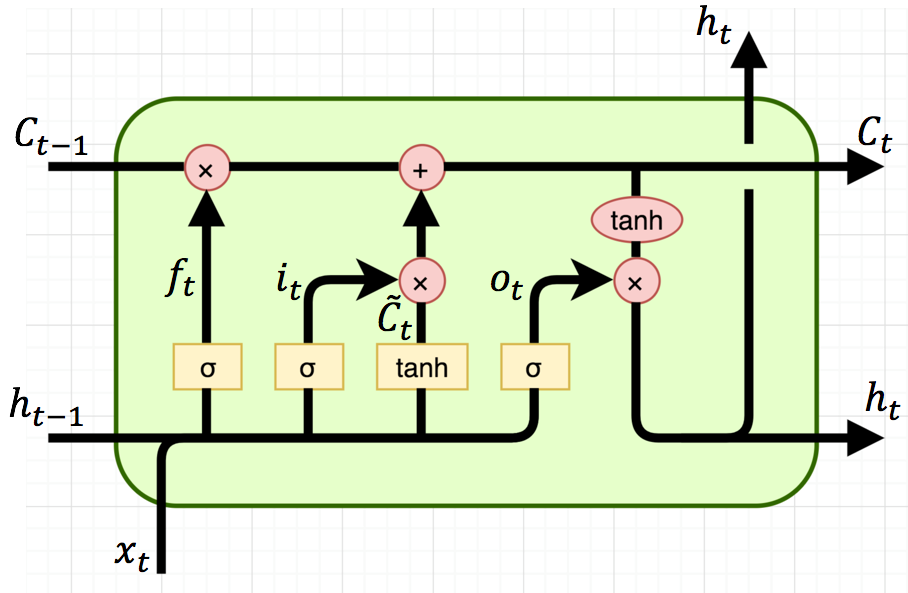
\includegraphics[width=\linewidth]{images/LSTM2.png}
	\caption{\textbf{LSTM Cell.} $x_t$ is cell input, $C_t$ is the current cell state, $h_t$ cell output.}
	\label{fig:lstm-cell}
\end{figure}
\par In the third stage we use the sigmoid function to check which part $O_t$ of the cell state our neuron outputs,
then that part is pre-processed with the tanh activation function and outputted.
The third stage is described in Equation~\ref{eqn:lstm-stage3}
\begin{equation}
	\begin{aligned}
    O_t &= \sigma(b_o + W_o x_t + U_o h_{t-1}), \\
    h_t &= O_t \times tanh(C_t).
    \end{aligned}
    \label{eqn:lstm-stage3}
\end{equation}
\par For our paper we used a many-to-one stacked stateless LSTM-ANN neural network. 
We used three LSTM layers followed by one ANN layer; all layers were comprised of 100 neurons.
For regularization a dropout rate of 0.2 was used and a weight decay of $l1=0.00001$, $l2=0.000001$.
We did not use Batch normalization for our LSTM model.
We normalized our data and used a lag window of size 60.
We trained our LSTM model for 200 epochs with pre-emptive stopping. 
\subsubsection{CNN}
\par For our second model we used a stacked 2D CNN-ANN. 
CNN models are commonly used to extract and combine hierarchical data from time series features~\cite{HOSEINZADE2019273}.
\par A convolutional layer is comprised of a filter applied to the input matrix $[v_{i,j}]$.
Each filter utilizes a shared set of weights to perform convolution, which are updated during training.
The filter output is feed into an activation unit. 
We used ReLU as our activation unit of choice for our CNN layers.
\par As our CNN input we created an image where the first dimension represented our $j$ stock features and the second the $i$ time lags.
In the first layer we combined our features with a 1d convolution layer with kernel size of six, in the second layer we combined our lags with a 1d convolution with kernel size three.
\begin{figure}[!ht]\centering
	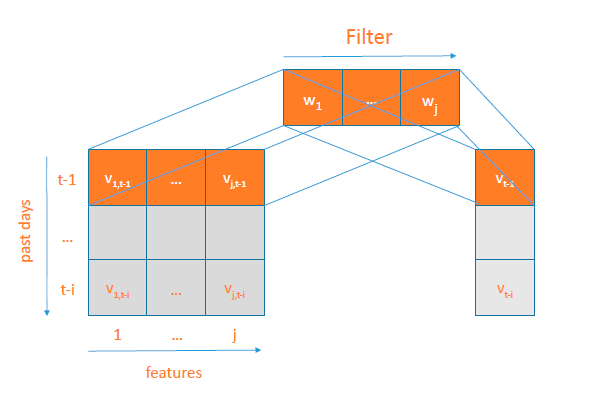
\includegraphics[width=\linewidth]{images/CNNpred.png}
	\caption{\textbf{2D CNN.} Extracting and combining data from features and lags.}
	\label{fig:cnn-pred}
\end{figure}
\par The formal transformation preformed by our convolutional layers in given by Equation~\ref{eqn:cnn-def}
\begin{equation}
	\begin{aligned}
    v_{i,j} = \delta(\Sigma^{F-1}_{k=0} \Sigma^{F-1}_{m=0} w_{k,m} V_{i+k,j+m}),
    \end{aligned}
    \label{eqn:cnn-def}
\end{equation}
where $V$ is the input image, $F$ is the symmetric filter size, $w$ are the filter weights and $\delta$ is the activation function.
\par We used a max polling layer to sub sample our data, in order to reduce the computational cost of our learning process as well as reduce overfitting.
%We also used Batch normalization in order to speed up training.
%Batch normalization is a set of additional network layers that reduces the internal covariance shift, this at a high level stabilizes the input %distribution from layer to layer. 
\par Our CNN is structured as follows: the first two layers are 1d Conv layers, followed by a maxpool layer, followed by 3 ANN layers with 100, 200 and 200 neurons respectively, after each layer we used batch normalization.
For regularization a dropout rate of 0.2 was used and a weight decay of $l1=0.0000001$, $l2=0.0000001$.
We standardized our data and used a lag window of size 18.
We trained our CNN model for 200 epochs with pre-emptive stopping.
\subsubsection{CNN-LSTM}
\par Our third and final model is the CNN-LSTM-ANN model which uses both CNN and LSTM layers. The Conv layers are used to capture hierarchical nonlinear data, while the LSTM layers are used to capture long-term dependencies in our data. The CNN-LSTM has been shown to outperform both LSTM and CNN~\cite{carbon}.
\par Unlike in the previous model the Conv layers are used exclusively to extract spatial temporal data and not to extract inter-feature information.
The CNN-LSTM structure is shown in figure~\ref{fig:cnn_lstm-def}.
\begin{figure}[H]\centering
	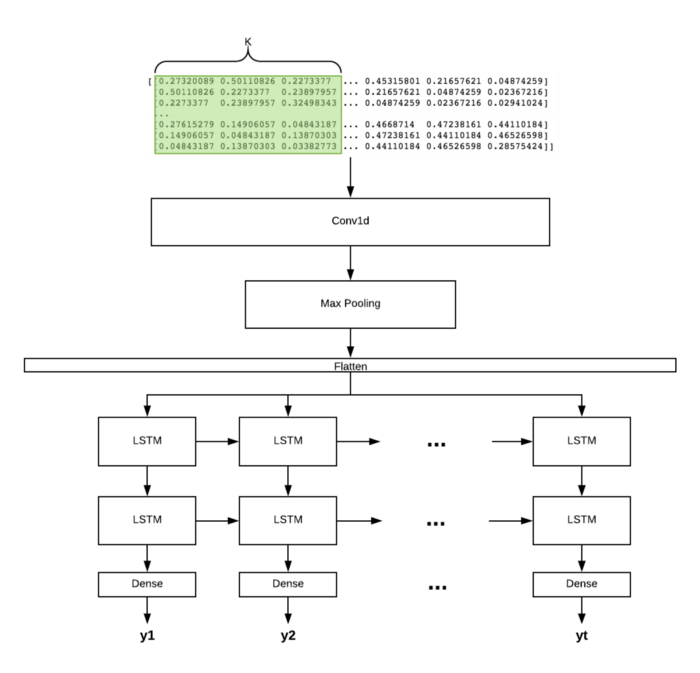
\includegraphics[width=\linewidth]{images/CNN_LSTM.png}
	\caption{\textbf{CNN-LSTM.} Extracted data from CNN is used in LSTM.}
	\label{fig:cnn_lstm-def}
\end{figure}
\par Our CNN-LSTM model was constructed as follows: our first two layers were 1d Conv layers  with kernel size three wrapped in the \textit{TimeDistributed} layer, following were two LSTM layers with 100 neurons each, followed by three ANN layers with 100 neurons each.
For regularization a dropout rate of 0.2 was used and a weight decay of $l1=0.0000001$, $l2=0.0000001$.
We standardized our data and used a lag window of size 18.
We trained our CNN-LSTM model for 500 epochs with pre-emptive stopping.
\subsection{Deseasonilizing \& detrending}
\par Most training models work better when the time series is stationarized and the data is deseasonalized and detrended.
We used the ARIMA model to remove the trend and seasonality of our time series.
For each data set we iteratively predicted the next-day values with ARIMA and then subtracted the result from our data gaining residuals. In order to test the stationarity of our time series we used the Augmented Dickey-Fuller (ADF) statistical test, achiving a p-value of 0.01 on all residual dataset. We then used our models to predict the residuals. We compared $RMSE$ to the original ARIMA $RMSE$; the $RMSE$ of our models residuals is the same as our $RMSE$ on the original datasets, therefore we can compare them.

\subsection{Model Explainability}
\par In order to explain our results we used Locally Interpretable Model-Agnostic Explanations~\cite{LIME} (LIME). 
LIME perturbs our sample data point $x$ in order to get perturbations $z^{'}$ which are then evaluated by an interpretable model $g$ which approximates our model $f(z)$, finally values $g(z^{'})$ are used to approximate our feature value $z$.
A model is considered interpretable if we can visually inspect our results and verify our assumptions about the model.
The current python implementation of LIME uses lines to explain models.
This does require our model to be locally linear.
The formal definition of LIME is given in Equation~\ref{eqn:lima-def}
\begin{equation}
	\begin{aligned}
    &\xi(x) = \underset{g \in G}\argmin \Lagr(f,g,\pi_x) + \Omega(g), \\
    &\Lagr(f,g,\pi_x) = \Sigma \pi_x(z)d(f(z),g(z^{'})),
    \end{aligned}
    \label{eqn:lima-def}
\end{equation}
where $\pi_x$ is probability of sampling point $z$ and $d$ is the cosine distance.
\par We aggregated the explanation to get marginal explanations for both features and lags. 
\subsection{Evaluation}
\par We evaluated our models using cross-validation on a rolling basis. Figure~\ref{fig:cros-val} show the core idea of cross-validation on a rolling basis. We picked 10 six year intervals shifted by half a year. In each interval the first five years were used for training and validation while the last year was used for model testing.
We used mean absolute percentage error (MAPE) for cross-model comparison and root mean squared error (RMSE) for an interpretable quantification of error.
For quantification of uncertainty standard deviation of absolute percentage error (SDAPE) was used, furthermore standard deviation for cross-validation was also calculated.
\begin{equation}
    \begin{aligned}
    &RMSE = \sqrt{\frac{1}{N}\Sigma^{N}_{i=1} (y_i - \hat{y}_i)^2}\\
    &MAPE = \frac{1}{N}\Sigma^{N}_{i=1} |{\frac{y_i - \hat{y}_i}{y_i}}|\\
    &SDAPE = \sqrt{\frac{1}{N}\Sigma^{N}_{i=1}(\frac{y_i - \hat{y}_i}{y_i} - MAPE)}\\
    \end{aligned}
\end{equation}

\begin{figure}[!ht]\centering
	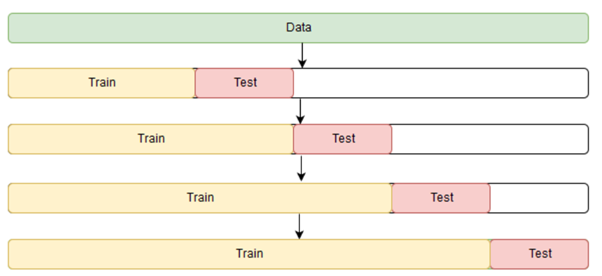
\includegraphics[width=\linewidth]{images/cros_validation.png}
	\caption{\textbf{Cross-validation on a rolling basis.} We trained our model on consecutive five year time periods and tested it on the following year time period.
	}
	\label{fig:cros-val}
\end{figure}

\subsection{Implementation details}
\par Our code was implemented in python. 
We used Keras to build all our neural network models and statsmodels for ARIMA and our Dickey-Fuller test.
For LIME we used the python LIME library and for result visualizations we used plotnine.

\section{Results}
\subsection{General results}
\par In Figure~\ref{fig:res1} we compared models based on mean MAPE and SDAPE.
\begin{figure}[!ht]\centering
	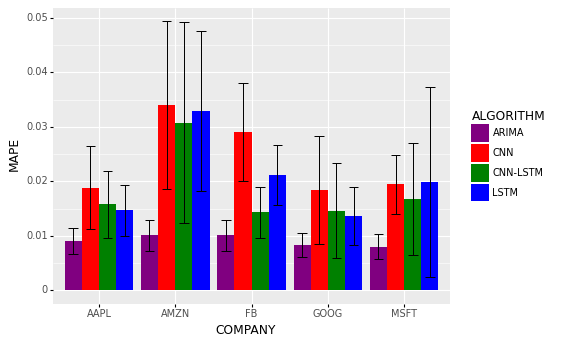
\includegraphics[width=\linewidth]{images/fig1.png}
	\caption{\textbf{MAPE across datasets.} The height of the bars represents mean MAPE with the lines representing SDAPE.}
	\label{fig:res1}
\end{figure}
\begin{table}[hbt]
	\caption{MAPE and RMSE of models.}
	\centering
	\begin{tabular}{|l|r|r|r|r|}
	    \hline
        \toprule
        ALGORITHM &  MAPE &  SDAPE &  RMSE &  SDMSE \\
        \hline
        \midrule
            ARIMA & 0.009 &  0.003 &  8.02 &   4.07 \\
              CNN & 0.024 &  0.009 & 17.26 &   8.64 \\
         CNN-LSTM & 0.018 &  0.010 & 13.96 &   8.45 \\
             LSTM & 0.020 &  0.010 & 16.12 &   8.96 \\
        \hline
        \bottomrule
    \end{tabular}
	\label{tab:res1}
\end{table}
We see that ARIMA scored on average the best accross all datasets. 
CNN appears to have scored consistently the worst.
From Figure~\ref{fig:res1}  and Table~\ref{tab:res1} we conclude that ARIMA is statistically the best scoring prediction model, while CNN is the worst.
We note that our results for CNN-LSTM and LSTM are inconclusive since despite CNN-LSTM scoring on average better than LSTM it did so inconsistently with LSTM being better on AAPL and GOOG.
In term of mean stability ARIMA is the most stable model, while the other models have comparable mean stability.

\subsection{Hybrid model comparison}
\par We removed the ARIMA predicted values from the datasets and trained our models on the residuals.
While this process changes MAPE significantly, it leaves RMSE intact therefore in the following section we will analyze RMSE change in comparison with the original ARIMA. 
This process also stationarized all five of our time series.
\begin{figure}[!ht]\centering
	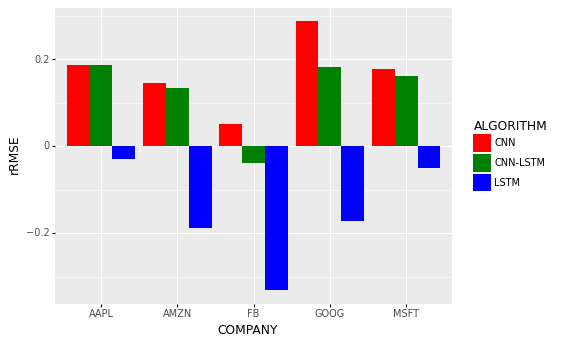
\includegraphics[width=\linewidth]{images/fig2.png}
	\caption{\textbf{RMSE normalized.} The following histogram represents the reduction in RMSE relative to ARIMA.}
	\label{fig:res2}
\end{figure}
\begin{table}[hbt]
	\caption{RMSE of residuals.}
	\centering
    \begin{tabular}{|l|r|r|r|r|r|r|}
    \toprule
    \hline
    {} &  AAPL &   AMZN &    FB &   GOOG & MSFT \\
    \hline
    \midrule
    ARIMA     &  0.64 &  22.11 &  2.59 &  13.52 &  1.26 \\
    %\hline
    CNN       &  0.57 &  20.27 &  2.54 &  11.93 &  1.11 \\
    %\hline
    CNN-LSTM  &  0.57 &  20.41 &  2.63 &  12.51 &  1.13 \\
    %\hline
    LSTM      &  0.65 &  24.48 &  2.92 &  14.47 &  1.30 \\
    \hline
    \bottomrule
    \end{tabular}
	\label{tab:res2}
\end{table}
\par From Table~\ref{fig:res2} and Figure~\ref{tab:res2} we see that the best model in ARIMA residual prediction is CNN, with CNN-LSTM being second,
while LSTM consistently increases the residual error.
We note that this is not because of incorrect hyperparameter tunning as the LSTM model displayed extremely erratic prediction patterns and failed to predict certain parts of the model entirely as can be observed from the results in Apendix A.
\subsection{Model Explainability}
\par In this section we used LIME to analyze our models and compare the importance they assign to features and to lags as well as how this changes when the models are trained on residuals.
\begin{figure}[!ht]\centering
	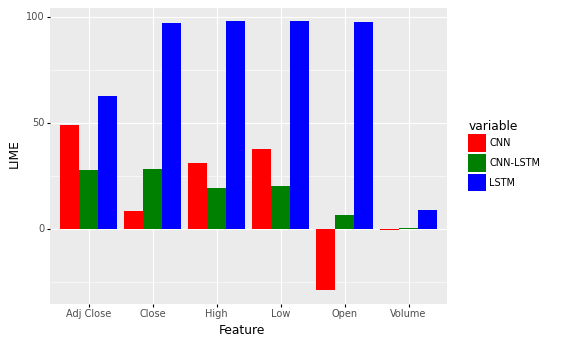
\includegraphics[width=\linewidth]{images/fig3.png}
	\caption{\textbf{LIME of features.} Histogram shows marginal feature importance.}
	\label{fig:expl1}
\end{figure}
As shown in Figure~\ref{fig:expl1} all three models assign almost no importance to Volume, this is inline with Wang et al~\cite{wang2003} who also found volume to be a poor predictor of stock growth.
LSTM assign importance nearly uniformly across all other variables, while CNN-LSTM appears to favour Adj Close and Close, this being more inline with our intuition as we would assume that the closing price being closer to the next-day opening price should be a better predictor than other prices.
While CNN does appear to assign high importance to Adj Close it assign little to Close and negative to Open, this is definitely unexpected as the Opening price should still be positively correlated with the next day price as such this might be the cause of CNNs poor performance.
We note that CNN assigns higher feature importance to Low compared to High, indicating perhaps that the lowest daily stock price is a better predictor of stock value than the highest daily stock price, however this is questionable considering CNNs poor prediction score.
\begin{figure}[!ht]\centering
	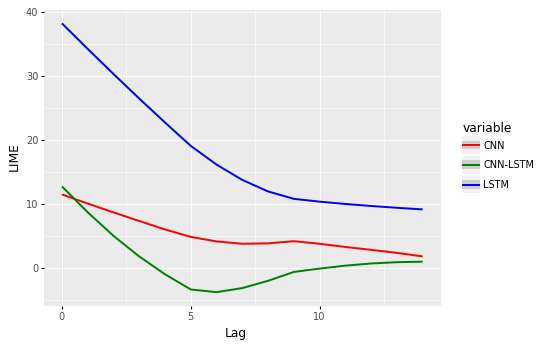
\includegraphics[width=\linewidth]{images/fig4.png}
	\caption{\textbf{LIME of lags.} Smoothed marginal importance of each lag; lag $n$ represent lag at $t-(n+1)$.}
	\label{fig:expl2}
\end{figure}
\par All three models appear to assign higher importance to earlier lags and lower importance to later lags, with CNN and CNN-LSTM approaching zero as lags grow above 12. 
This is inline with our empirical results achieved during parameter tunning, where we found that both CNN and CNN-LSTM performed poorly with bigger lag windows, whereas LSTMs were shown to be much more resilient; considering LSTM scored similarly to CNN-LSTM we conclude that LSTM might have been assigning to much importance to later lags.
Another interesting observation is the CNN-LSTM inflection around lag five. It appears that CNN-LSTM assumed that lags between three and eight are anti-correlated with the next day stock value.
\begin{figure}[!ht]\centering
	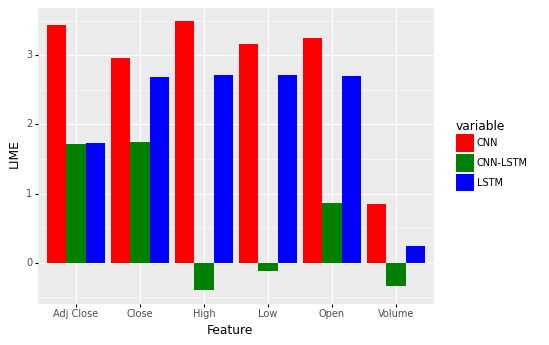
\includegraphics[width=\linewidth]{images/fig5.png}
	\caption{\textbf{Lime of residual features.} Histogram shows marginal feature importance.}
	\label{fig:expl5}
\end{figure}
\par In Figure~\ref{fig:expl5} we compare LIME of residual features.
Despite CNN being the best predictor and LSTM the worst, the overall distribution of importance appears to be similar for LSTM and CNN, with the clear exception that CNN adds far more importance to Adj Close, wheres LSTM appears to distribute feature importance almost uniformly.
\par CNN-LSTM by distribution completely diverges from LSTM and CNN. It assigns near-zero importance to most features besides Close, Adj Close and Open. It is possible that CNN-LSTM found another important relationship in our data different from the first two, however further analysis is necessary to make a conclusion. 
\begin{figure}[!ht]\centering
	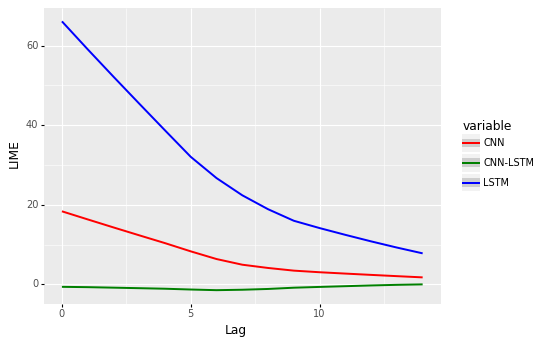
\includegraphics[width=\linewidth]{images/fig6.png}
	\caption{\textbf{LIME of residual lags.} Smoothed marginal importance of each lag; lag $n$ represent lag at $t-(n+1)$.}
	\label{fig:expl6}
\end{figure}
\par From Figure~\ref{fig:expl6} we conclude that CNN-LSTM was most likely unable to properly learn from the dataset as its lag importance is close to zero for all lags. 
Figure~\ref{fig:expl6} also provides an explanation why LSTM underperformed in comparison to CNN; ARIMA removed a significant amount of long term dependencies, considering the uniformly high overall lag importance assigned by LSTM we conclude it improperly modeled the temporal features of our time series. 
Another noteworthy observation is that both LSTM and CNN have very similair lag graphs for both residuals and the original dataset, while this is expected in the case of CNN it is far less expected in the instance of LSTM. %, which should have cell state weights trained during intra-batch training.
\section{Conclusion}
\par We have on the problem of next-day stock prediction compared LSTM, CNN and CNN-LSTM and found that they consistently underperformed ARIMA both in mean prediction accuracy as well as in prediction stability, which is inline with other similar research~\cite{carbon}.
\par On the problem of residual training CNN was the best predictor. 
This finding is important as it is not inline with conventional wisdom to use either LSTM or CNN-LSTM to model time series residuals~\cite{carbon}. 
It also implies that ARIMA is able to remove a significant portion of long term dependencies. 
All models were analyzed by LIME, which we showed to be a very powerful tool for model analysis, as it was able to explain the poor residual predictions of LSTM as well as discover CNN-LSTMs failure to properly model residuals. 

% if have a single appendix:
%\appendix[Proof of the Zonklar Equations]
% or
%\appendix  % for no appendix heading
% do not use \section anymore after \appendix, only \section*
% is possibly needed

% use appendices with more than one appendix
% then use \section to start each appendix
% you must declare a \section before using any
% \subsection or using \label (\appendices by itself
% starts a section numbered zero.)
%


% use section* for acknowledgement
\ifCLASSOPTIONcompsoc
  % The Computer Society usually uses the plural form
  \section*{Acknowledgments}
\else
  % regular IEEE prefers the singular form
  \section*{Acknowledgment}
\fi


The authors would like to thank the professors and assistants of the Faculty of Computer Science for providing us with the knowledge necessary to write this paper.


% Can use something like this to put references on a page
% by themselves when using endfloat and the captionsoff option.
\ifCLASSOPTIONcaptionsoff
  \newpage
\fi



% trigger a \newpage just before the given reference
% number - used to balance the columns on the last page
% adjust value as needed - may need to be readjusted if
% the document is modified later
%\IEEEtriggeratref{8}
% The "triggered" command can be changed if desired:
%\IEEEtriggercmd{\enlargethispage{-5in}}

% references section

% can use a bibliography generated by BibTeX as a .bbl file
% BibTeX documentation can be easily obtained at:
% http://www.ctan.org/tex-archive/biblio/bibtex/contrib/doc/
% The IEEEtran BibTeX style support page is at:
% http://www.michaelshell.org/tex/ieeetran/bibtex/
%\bibliographystyle{IEEEtran}
% argument is your BibTeX string definitions and bibliography database(s)
%\bibliography{IEEEabrv,../bib/paper}
%
% <OR> manually copy in the resultant .bbl file
% set second argument of \begin to the number of references
% (used to reserve space for the reference number labels box)
%\begin{thebibliography}{1}

%\bibitem{IEEEhowto:kopka}
%H.~Kopka and P.~W. Daly, \emph{A Guide to {\LaTeX}}, 3rd~ed.\hskip 1em plus
%  0.5em minus 0.4em\relax Harlow, England: Addison-Wesley, 1999.

%\end{thebibliography}

\bibliographystyle{IEEEtran}
\bibliography{report}

% biography section
% 
% If you have an EPS/PDF photo (graphicx package needed) extra braces are
% needed around the contents of the optional argument to biography to prevent
% the LaTeX parser from getting confused when it sees the complicated
% \includegraphics command within an optional argument. (You could create
% your own custom macro containing the \includegraphics command to make things
% simpler here.)
%\begin{IEEEbiography}[{\includegraphics[width=1in,height=1.25in,clip,keepaspectratio]{mshell}}]{Michael Shell}
% or if you just want to reserve a space for a photo:

% if you will not have a photo at all:

% insert where needed to balance the two columns on the last page with
% biographies
%\newpage

% You can push biographies down or up by placing
% a \vfill before or after them. The appropriate
% use of \vfill depends on what kind of text is
% on the last page and whether or not the columns
% are being equalized.

%\vfill

% Can be used to pull up biographies so that the bottom of the last one
% is flush with the other column.
%\enlargethispage{-5in}



% that's all folks
\end{document}


